\section{Suslin Trees} \label{Ch5:Sec:Suslin_Trees}

We now return to the setting of Suslin's problem (\Cref{Ch5:Sec:Suslin}), and to trees of height $\omega_1$.

\subsection{Characterising Suslin Trees}

% The raw notes break off here, between antichains and diamond, with the two comments below. None of the board photographs supplied with the post-lecture pass of 6 Nov 2026 covers this part, so the definition of a Suslin tree (which the lemma below uses) and the statement of Jensen's theorem given here are both missing.
% fill in from phone pictures
% state jensen's theorem
\sorry

Suslin trees are characterised by their antichains.

\begin{boxlemma}
    $\parenth{T, <_{T}}$ is a Suslin tree iff it's a normal $\omega_1$-tree with no uncountable antichain.
\end{boxlemma}

\subsection{A Suslin Tree from $\Diamond$}

We now construct a Suslin tree from a $\Diamond$-sequence.

\begin{boxconstruction}[Constructing a Suslin Tree from a Diamond]
    Fix a $\Diamond$-sequence $\grpres{A_{\alpha}}{\alpha < \omega_1}$. By recursion, we'll build trees $\parenth{T_{\alpha}, <_{\alpha}}$ indexed by ordinals $\alpha < \omega_1$. We'll maintain:
    \begin{enumerate}
        \item $T_{\alpha}$ is a tree of height $\alpha$
        \item $T_{\alpha}$ as a set (not as a tree) is a countable ordinal. In fact, $\alpha \leq T_{\alpha} < \omega_1$
        \item For $\alpha < \beta < \omega_1$, $T_{\alpha}$ is end-extended by $T_{\beta}$ (trees) in the ``strong sense'':
        \begin{enumerate}
            \item $<_{\alpha} \ssq <_{\beta}$
            \item for every $\eta < \alpha$, $\level_{\eta}\of{T_{\alpha}} = \level_{\eta}\of{T_{\beta}}$
        \end{enumerate}
    \end{enumerate}
    The plan is to define $\parenth{T, <_T}$ to be the union of the $\parenth{T_{\alpha}, <_{\alpha}}$s and get that $\parenth{T, <_T}$ is a Suslin tree, but other things need to hold for this. \\

    Consider the base case
    \begin{align*}
        \parenth{T_0, <_0} = \parenth{0, \emptyset}
    \end{align*}
    Define $\parenth{T_1, <_1} := \parenth{\set{0}, \emptyset}$. We want to define $T_2$ to be the tree with root $0$ and children $1$ and $2$. Or something like that. So define
    \begin{align*}
        \parenth{T_2, <_2} := \parenth{\set{0, 1, 2}, \set{(0, 1), (0, 2)}}
    \end{align*}
    \begin{figure}[H]
        \centering
        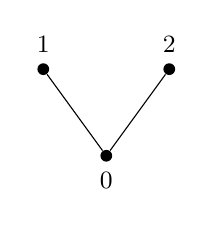
\begin{tikzpicture}[dot/.style = {circle, fill, inner sep = 1.5pt}, every node/.style = {font = \small}, grow' = up, level distance = 1.1cm, sibling distance = 1.6cm]
            \node[dot, label = {below:$0$}] {}
                child {node[dot, label = {above:$1$}] {}}
                child {node[dot, label = {above:$2$}] {}};
        \end{tikzpicture}
    \end{figure}
    In similar fashion, we define $T_3$ to be the tree extending $T_2$ with the children of $1$ being $3$ and $4$ and the children of $2$ being $5$ and $6$.
    \begin{figure}[H]
        \centering
        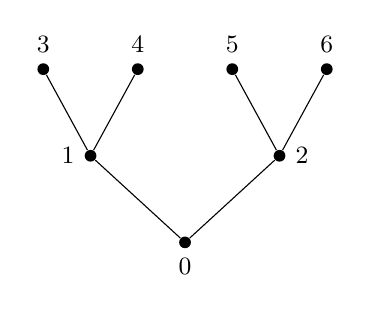
\begin{tikzpicture}[dot/.style = {circle, fill, inner sep = 1.5pt}, every node/.style = {font = \small}, grow' = up, level distance = 1.1cm, level 1/.style = {sibling distance = 2.4cm}, level 2/.style = {sibling distance = 1.2cm}]
            \node[dot, label = {below:$0$}] {}
                child {node[dot, label = {left:$1$}] {}
                    child {node[dot, label = {above:$3$}] {}}
                    child {node[dot, label = {above:$4$}] {}}}
                child {node[dot, label = {right:$2$}] {}
                    child {node[dot, label = {above:$5$}] {}}
                    child {node[dot, label = {above:$6$}] {}}};
        \end{tikzpicture}
    \end{figure}
    This is how we define successor trees. \\

    % Transcribed from the board photographs.
    % [CORRECTED] was: ``can be listed as $\xi_n$ for $n < \omega$'' and ``is $T_{\gamma} + \omega$'', for every $\beta$ --- when $\beta$ is finite the level has $2^{\beta}$ nodes and $T_{\delta} = T_{\gamma} + 2^{\beta + 1}$ (eg $T_3 = 7$, not $\omega$)
    Now consider the successor of a successor level. Say $\delta = \gamma + 1 = \parenth{\beta + 1} + 1$. How do we define $\parenth{T_{\delta}, <_{\delta}}$ based on $\parenth{T_{\gamma}, <_{\gamma}}$? We know (by the recursion hypothesis) that the universe of $T_{\gamma}$ is a countable ordinal. So $\level_{\beta}\of{T_{\gamma}}$ can be listed as $\xi_n$ for $n < \omega$ (for $n < 2^{\beta}$, if $\beta$ is finite). Define $T_{\delta}$ by putting $T_{\gamma} + 2n$ and $T_{\gamma} + 2n + 1$ above $\xi_n$.
    \begin{figure}[H]
        \centering
        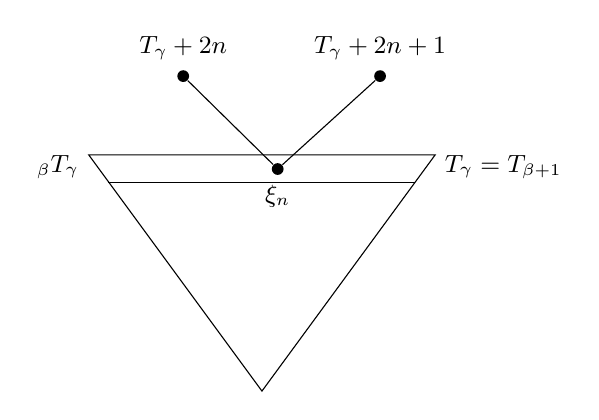
\begin{tikzpicture}[dot/.style = {circle, fill, inner sep = 1.5pt}, every node/.style = {font = \small}]
            \draw (0, 0) -- (-2.2, 3) -- (2.2, 3) -- cycle;
            \draw (-1.95, 2.65) -- (1.95, 2.65);
            \node[left] at (-2.2, 2.85) {$\level_{\beta}\of{T_{\gamma}}$};
            \node[right] at (2.2, 2.85) {$T_{\gamma} = T_{\beta + 1}$};
            \node[dot, label = {below:$\xi_n$}] (x) at (0.2, 2.82) {};
            \node[dot, label = {above:$T_{\gamma} + 2n$}] (y) at (-1, 4) {};
            \node[dot, label = {above:$T_{\gamma} + 2n + 1$}] (z) at (1.5, 4) {};
            \draw (x) -- (y);
            \draw (x) -- (z);
        \end{tikzpicture}
    \end{figure}
    We see that $T_{\delta}$ (the universe) is $T_{\gamma} + \omega$ (or $T_{\gamma} + 2^{\beta + 1}$, if $\beta$ is finite, as with $T_2$ and $T_3$). \\

    At every limit ordinal $\beta < \omega_1$, define
    \begin{align*}
        \parenth{T_{\beta}, <_{\beta}} := \parenth{\bigcup_{\alpha < \beta} T_{\alpha}, \bigcup_{\alpha < \beta} <_{\alpha}}
    \end{align*}
    In particular, we now know $\parenth{T_{\omega}, <_{\omega}}$. It's easy to see that $\parenth{T_{\omega}, <_{\omega}} \simeq {^{<\omega}2}$.

    % Transcribed from the board photographs.
    All that remains is
    \begin{enumerate}
        \item how to define $\parenth{T_{\delta}, <_{\delta}}$ when $\delta = \gamma + 1$ and $\gamma$ is a limit ordinal, and
        \item why it works.
    \end{enumerate}
    % The lecture stopped here, at ``All that remains is. Still owed: the successor-of-a-limit step, which is where the $\Diamond$-sequence is used, and the proof that the union is a Suslin tree. Normality is not among the three invariants listed above, but the construction will need it (it is what makes each level from $\omega$ on countably infinite, which the successor-of-a-successor step assumes).
    \sorry
\end{boxconstruction}
